\chapter{Interferometry, Calibration \& Polarimetry}
\label{chapter:interferometry}

In this Chapter I wished to build a formalism around wide-field, polarized interferometric measurements that could be used throughout this work. Many traditional assumptions used in radio interferometry are broken in the case of the wide-field, fully-polarized, drift-scanning measurements native to interferometric EoR observations. In Section~\ref{sec:interferometry_vis}, I derive the equation describing the fundamental observable for an interferometer, called a ``visibility". Section~\ref{sec:interferometry_cal}, I describe calibration techniques relevant to this work and in Section~\ref{sec:interferometry_pol} I review some of the implications of the previous two sections for polarized measurements.

For a comprehensive review of interferometry from a traditional perspective, see \cite{TMS}.

\section{The Visibility Equation}
\label{sec:interferometry_vis}

A radio interferometer (a term used interchangeably with ``interferometric array" for radio observations) is an ensemble of receiving elements, where each element's measurement is correlated with every other element's. The simplest case is a two-element interferometer, which we will focus on below. We assume that the elements are coplanar and identical.

\subsection{The Classical Visibility Equation}

Consider two receiving elements $i$ and $j$, separated by baseline vector $\vec{b}$. Suppose a plane wave of wavelength $\lambda$ is incident upon these elements, with direction of propagation $-\hat{s}$. The geometry of this interferometer is illustrated in Figure~\ref{fig:interferometry_2element}.

\begin{figure}
\centering
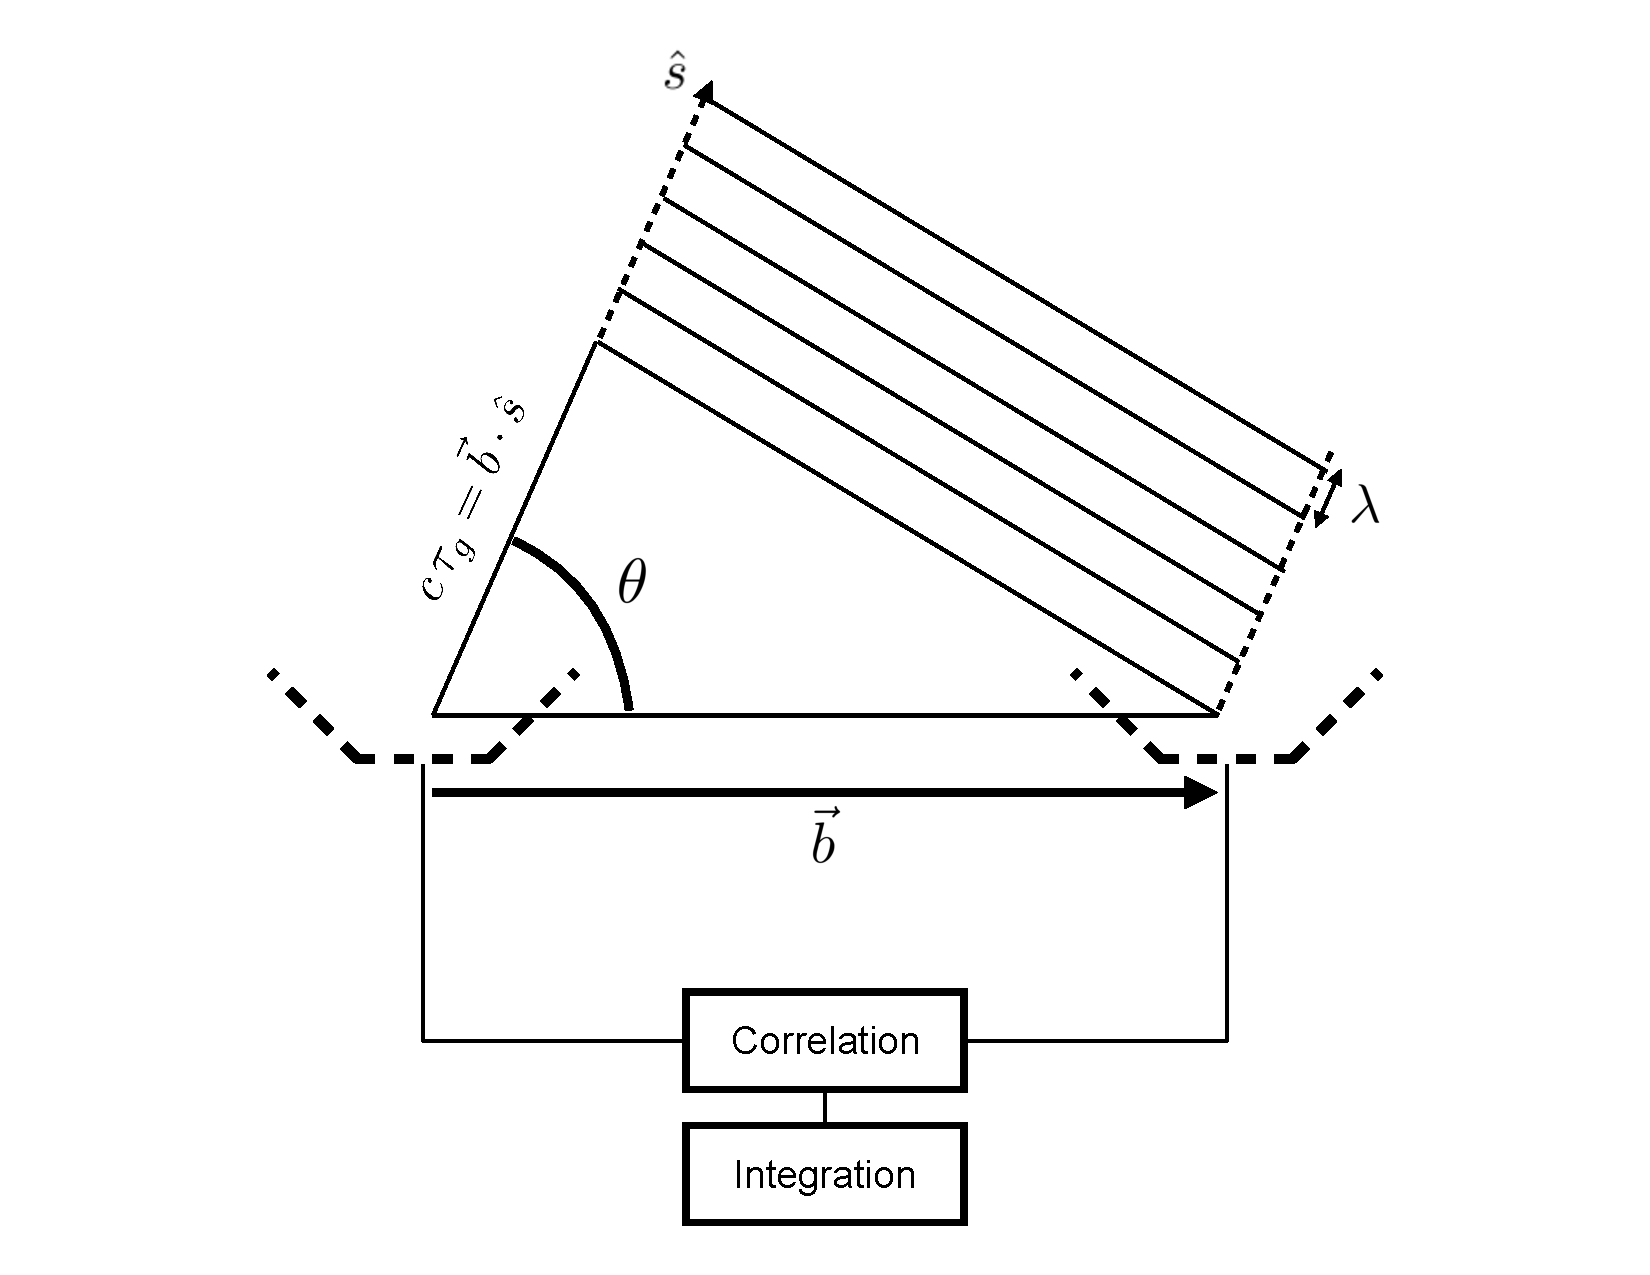
\includegraphics[width=0.9\textwidth]{chapters/interferometry/figures/visibility_explanation.pdf}
\caption{The geometry of a two-element interferometer, with a plane wave incident from direction $\hat{s}$.}
\label{fig:interferometry_2element}
\end{figure}

We can define the electromagnetic wave to have a frequency dependent phase, such that the electric field measured by element $i$ at time $t$ is

\begin{equation}
E_i = E_0 e^{-2\pi i \nu t}.
\label{eq:Ei}
\end{equation}

The time difference between the arrival at $i$ and $j$ is called the ``geometrical delay", $\tau_g$:

\begin{equation}
\tau_g = \frac{\vec{b}\cdot\hat{s}}{c},
\end{equation}
and the electric field measured by element $j$ is

\begin{equation}
E_j = E_0 e^{-2\pi i \nu (t+\tau_g)}.
\end{equation}

An interferometer is an instrument which measured voltages induced by these electric fields, and correlates them together, integrating their product over some coherent time-scale. This correlation grants:

\begin{equation}
\langle E_i E_j^* \rangle 
= \lim_{T\rightarrow\inf}\frac{1}{2T}\int^T_{-T} E_i(t) E_j(t) {\rm d}t
= | E_0 |^2 e^{-2\pi i \nu \tau_g}
\label{eq:vis_time_integration}
\end{equation}
where $e^{-2\pi i \nu \tau_g} = e^{-2\pi i \nu \vec{b}_{ij}\cdot\hat{s}/c}$ is known as the ``fringe" term, due to its sinusoidal nature. We can generalize this relationship to include more than a single plane wave from direction $\hat{s}$. Many plane waves, from all directions, can be incident upon the interferometer at a given time and frequency. We can represent the power distribution on the sky as $S(\Omega)$, where $S(\Omega)$. However, no instrument is equally sensitive to radiation from every direction $\hat{s} \in \Omega$. Instead, an instrument has some sensitivity pattern -- a \textit{beam pattern} -- that tapers the power distribution on the sky into an ``observed sky",  $S'(\Omega) = A(\Omega)S(\Omega)$. 

These generalizations lead to the classical visibility equation:

\begin{equation}
V_{ij}(\nu) = \int A(\Omega, \nu) S(\Omega, \nu) e^{-2\pi i \nu \vec{b}_{ij}\cdot\hat{s}/c} {\rm d}\Omega
\label{eq:classical_visibility}
\end{equation}
for a ``visibility" -- the fundamental interferometric observable -- $V_{ij}$ as a function of frequency.

If we choose to represent the source direction in terms of directional cosines $\ell$ and $m$, and represent the baseline vector in units of wavelengths, $\vec{b}_{ij}/\lambda=(u,v,w)$, we can perform a change of variables in Equation~\ref{eq:classical_visibility} to give

\begin{equation}
V_{ij}(u,v) = \int\int A(\ell, m)S(\ell, m) e^{-2\pi i (u\ell + vm + w\sqrt{1 - \ell^2 - m^2})} \frac{ {\rm d}\ell {\rm d}m }{\sqrt{1 - \ell^2 - m^2}}.
\label{eq:vis_def_widefield}
\end{equation}

This relationship is often simplified by assuming only a small area of the sky is under observation -- that is, that $A(\ell,m)$ falls-off steeply from zenith -- and therefore $\ell^2$ and $m^2$ are small. This grants

\begin{equation}
V_{ij}(u,v) \approx e^{-2\pi i w} \int\int A(\ell, m)S(\ell, m) e^{-2\pi i (u\ell + vm)} {\rm d}\ell {\rm d}m,
\label{eq:vis_dev_narrowfield}
\end{equation}
which plainly casts $V(u,v)$ as the Fourier transform of the observed sky if $w$ is small: that is, the array is co-planar and no appreciable curvature of the sky is probed. Modern low frequency interferometers used in this work greatly violate this approximation, the consequences of which I will discuss in the proceeding sections.

Even though it is often violated, the Fourier relationship shown in Equation~\ref{eq:vis_dev_narrowfield} is an extremely useful one to work with when translating between visibilities and images. Images can be created by inverse Fourier transforming all of the visibilities measured by an array. Following Equation~\ref{eq:vis_def_widefield}, a reconstructed image $\tilde{S}(\ell, m)$ is given by

\begin{equation}
\frac{A(\ell, m)\tilde{S}(\ell, m)}{\sqrt{1 - \ell^2 - m^2}} = \int\int \Xi(u, v) V(u,v) e^{2\pi i \nu (u\ell + vm)} {\rm d}u {\rm d}v.
\label{eq:image_estimate}
\end{equation}

In Equation~\ref{eq:image_estimate}, we see that the reconstructed image $\tilde{S}(\ell, m)$ is attenuated by the beam response $A(\ell, m)/\sqrt{1 - \ell^2 - m^2}$. The function $\Xi(u, v)$ defines the sampling of the $u,\,v$ - plane. It is equal to 1 at the points sampled by the interferometer (baselines of length and direction defined by the vector  $\vec{b} = (u,v)$ exist in the array) and 0 elsewhere. As an example, the ``array" shown in Figure~\ref{fig:interferometry_2element} would be described by a $\Xi(u, v)$ function that was zero at all points except for a single ($u,\,v$) coordinate described by baseline vector $\vec{b}$.

The effect of the sampling function $\Xi(u, v)$ is that the true sky $S(\ell,m)$ can never be completely reconstructed, since it is impossible to build an interferometer that samples every $u,v$ mode. The true sky is convolved with the Fourier transform of $\Xi(u, v)$, which astronomers refer to as the ``dirty beam". $\Xi(u, v)$ contains zeros, so a complete deconvolution of $\tilde{S}(\ell, m)$ is impossible.

We now note that an important aspect of light has been absent throughout the derivations above: the polarization state of the radio wave that induces the electric field in Equation~\ref{eq:Ei}. Interferometers are typically constructed with two feeds, sensitive to polarization states of an incident radio wave along two separate axes. In the case of all of the instruments used in this work (see Chapter~\ref{chapter:instruments}), an antenna $i$ had two dipole feeds perpendicular to one another. These were along the North-South direction (`n') and the East-West direction (`e'). We can attempt to generalize Equation~\ref{eq:classical_visibility} to include polarization, setting antenna $i$ to have orientation $p$ and antenna $j$ to have orientation $q$, $p,q\in(e,n)$:

\begin{equation}
V^{pq}_{ij} = \int A_{pq}(\Omega, \nu) S_{pq}(\Omega, \nu) e^{-2\pi i \nu \vec{b}_{ij}\cdot\hat{s}/c} {\rm d}\Omega.
\end{equation} 
However, two aspects of this equation are unsatisfactory. As explored in Chapter~\ref{chapter:astro_rad}, the polarized sky is defined with the four Stokes parameters; an ``$S_{pq}$" polarized sky does not exist. Likewise, a dipole is not purely sensitive to a single vector orientation from the sky, but probes a wide range of angles\footnote{In the case of the PAPER instrument, described in the next Chapter, the dipole feeds probed the entire hemisphere of the sky.}. Therefore a $A_{pq}$ polarized beam is ill-defined. These shortcomings lead us to rewrite the visibility equation, cohesively including polarization from the outset.  

\subsection{The Measurement Equation}

The Radio Interferometric Measurement Equation (RIME) provides an extremely useful framework for describing wide-field polarized observations. Formulated by \cite{HBS.1.96}, it was re-introduced to the radio astronomy community through a series of papers by O.~M. Smirnov \citep{Smirnov.11, Smirnov.11.2, Smirnov.11.3, Smirnov.11.4}. In this section I review the portions of his work most relevant to this thesis, and defer the reader to the series for a useful and thorough walk-through of wide-field radio interferometry and high dynamic-range calibration.

Returning to Equation~\ref{eq:Ei}, a radio wave incident on an antenna induces a voltage in along feed arm

\begin{equation}
\vec{E} = (e_p, e_q);\,\,\,\vec{v} = (v_p,v_q) = \textbf{J}\vec{E}
\label{eq:voltage_jones}
\end{equation}
where \textbf{J} is a $2\times2$ complex matrix termed the ``Jones matrix" \citep{Jones.41}. Jones matrices represent linear transformations along the signal path, from the emission of the radio wave onwards. Multiple stages along the signal propagation can be represented by multiplying different Jones matrices together as a ``Jones chain", which may be expanded or collapsed as convenient.

Interferometric visibilities are pairwise correlations of the components of $\vec{v}$ between antennas $i$ and $j$, integrated over some small time span (Equation~\ref{eq:vis_time_integration}), which we can represent hold in matrix form (the layout of which will become clear in a moment):

\begin{equation}
\textbf{V}_{ij} = \begin{pmatrix} 
\langle v^p_i v^{p*}_j \rangle & \langle v^p_i v^{q*}_j \rangle \\
\langle v^q_i v^{p*}_j \rangle & \langle v^q_i v^{q*}_j \rangle \\
 \end{pmatrix} = \langle \vec{v}_i \vec{v}^H_j \rangle.
\end{equation}
Above, H represents the Hermitian transpose operation.

Using this formalism allows us to map the emitted electric field to the observed visibilities, 
\begin{equation}
\textbf{V}_{ij} = \textbf{J}_i \begin{pmatrix} 
\langle e^p_i e^{p*}_j \rangle & \langle e^p_i e^{q*}_j \rangle \\
\langle e^q_i e^{p*}_j \rangle & \langle e^q_i e^{q*}_j \rangle \\
 \end{pmatrix} \textbf{J}^H_j = \textbf{J}_i \textbf{C}_{ij} \textbf{J}^H_j
\end{equation}
where \textbf{J}$_{i,j}$ may be Jones chains of arbitrary length. We have assumed instrument stability to move them out of the time averages in the central matrix. We refer to $\textbf{C}_{ij}$ as the ``coherency matrix". 

In Chapter~\ref{chapter:astro_rad} the Stokes parameters we introduced. \cite{Hamaker-Bregman.96} showed that the components of the coherency matrix are closely related to the Stokes parameters:

\begin{equation}
\begin{pmatrix} 
\langle e^p_i e^{p*}_j \rangle & \langle e^p_i e^{q*}_j \rangle \\
\langle e^q_i e^{p*}_j \rangle & \langle e^q_i e^{q*}_j \rangle \\
 \end{pmatrix}
 =
 \begin{pmatrix} 
I + Q & U + iV \\
U - iV & I - Q \\
 \end{pmatrix}.
 \label{eq:interferometry-stokes-coherency}
\end{equation}

The Jones formalism allows for a construction of the visibility equation that does not make explicit assumptions regarding polarization or field-of-view, in which we can map the Stokes parameters into the instrumental basis that visibilities are computed in:

\begin{equation}
\textbf{V}_{ij} = \int \textbf{J}_i(\hat{s}) \textbf{C}_{ij}(\hat{s}) \textbf{J}_j^H(\hat{s}) e^{-2\pi i \nu \vec{b}_{ij}\cdot\hat{s}/c} {\rm d}\Omega,
\label{eq:RIME}
\end{equation}
which \cite{Smirnov.11} refers to as the ``Full Sky Radio Interferometric Measurement Equation"\footnote{We choose to explicitly show the exponent in this formulation for ease of comparison with Equation~\ref{eq:classical_visibility}. \cite{Smirnov.11} shows that this term can written as a ``phase delay Jones matrix" and absorbed into the Jones chain.}. Note that all of these quantities are functions of frequency as well, in general.

So far, the formalism shown has used the $2\times 2$ ``Jones basis". It is sometimes more useful to work in the $4\times 4$ ``Mueller basis" \citep{Mueller.48}, which acts on visibilities in $4\times 1$ vector form:

\begin{equation}
\begin{pmatrix}
V^I \\
V^Q \\
V^U \\
V^V \\
\end{pmatrix}
=
\textbf{S}\vec{V}_{ij}
= 
\begin{pmatrix}
1 & 0 & 0 & 1 \\
-1 & 0 & 0 & 1\\
0 & 1 & 1 & 0 \\
0 & -i & i & 0 \\
\end{pmatrix}
\begin{pmatrix}
V^{pp} \\
V^{pq} \\
V^{qp} \\
V^{qq} \\
\end{pmatrix}.
\label{eq:interferometry_pseudo_stokes}
\end{equation} 

It is important to note that Equation~\ref{eq:interferometry_pseudo_stokes} lists a vector of ``Stokes-polarized visibilities" on the left-hand side, whereas  Equation~\ref{eq:interferometry-stokes-coherency} shows that the coherency matrix contains linear combinations the Stokes parameters. This is not an inconsistency. While visibilities are quantities that are integrated over the sky, the Stokes parameters are only defined \textit{on} the sky. One must transform the visibilities from the $uv$-plane onto the image-plane and deconvolve the beam in order to measure the Stokes parameters. Instead, linear combinations of visibilities measure a proxy for each the Stokes parameters. To make the inequality between visibilities and Stokes parameters explicit, I will refer to the ``Stokes-polarized visibilities" as ``pseudo-Stokes visibilities" from now on.

One can translate between these two formalisms using the definition of $\vec{V}_{ij}$ (c.f. Equation~\ref{eq:voltage_jones}),

\begin{equation}
\vec{V}_{ij} = (\textbf{J}_i \otimes \textbf{J}_j^H)(\vec{E}\otimes\vec{E}^H).
\end{equation}

Comparison of Equation~\ref{eq:classical_visibility} and \ref{eq:RIME} shows that the Jones chain must, at the very least, encapsulate the beam pattern of the instrument. We can build such a Jones matrix by considering the response of feed $p$ on antenna $i$ to an electric field from infinity in the direction ($\theta$, $\phi$):

\begin{equation}
\vec{A}_i^p(\hat{s}) = A^p_{i,\theta}(\hat{s})\hat{\theta} + A^p_{i,\phi}(\hat{s})\hat{\phi},
\end{equation}
where we have suppressed the frequency dependence. The antenna patterns may be written as components of a ``Beam Jones matrix" for an antenna,

\begin{equation}
\textbf{J}_i^{\rm B}(\hat{s}) = 
\begin{pmatrix}
A^p_{i,\theta}(\hat{s}) & A^p_{i,\phi}(\hat{s}) \\
A^q_{i,\theta}(\hat{s}) & A^q_{i,\phi}(\hat{s}) \\
\end{pmatrix}.
\label{eq:jones-beam}
\end{equation}

These are the essential components for understanding the fundamental measurement performed by an interferometer. However, there are several effects one must take into account for the equations to truly reflect an interferometric measurement; effects such as instrumental gains, reflections between antennas, Faraday rotation in the ionosphere, etc. Most importantly, we must consider how these factors affect the measurement of polarization.

\section{Calibration Techniques}
\label{sec:interferometry_cal}

The purpose of calibration is to remove effects of the instrument and the atmosphere from the data. Visibilities are measured in ``data units". That is, a given feed on an antenna will record some measurement of power, but some scalar conversion factor is required to calibrate that power to units of flux density. As visibilities measure the pairwise correlations of antenna powers, the estimation of the calibration factors can quickly become difficult as the number of antennas increases. In this Section we explain different approaches to such a challenge.

\subsection{Diagonal and off-diagonal calibration}

The calibration term that converts the power measured by an antenna to physical units is referred to as the ``antenna gain". This may be summarized per feed as a direction-independent ``Gain Jones matrix",

\begin{equation}
\textbf{J}_i^{\rm G} = 
\begin{pmatrix}
g_i^p &0 \\
0 & g_i^q\\
\end{pmatrix},
\label{eq:jones-gains}
\end{equation}
where we have suppressed the frequency dependence. The components of $\textbf{J}_i^{\rm G}$ are complex numbers, the argument of which represents instrumental phase, and the modulus represents instrumental amplitude. Note that this formulation of $\textbf{J}_i^{\rm G}$ is only appropriate for linear antenna feeds. Circular feeds, which we will not comment on for the rest of this work, require an additional rotation matrix applied to move from a linear to a circular polarization frame.

Unfortunately, a direction-independent scaling is not the only term that requires estimation. As Equation~\ref{eq:jones-beam} makes clear, a given feed is not receptive to a single plane of polarization. In general, we expect some fraction of power measured by feed $p$ to be transferred into feed $q$ via imperfect electronics \citep[clever feed designs can attempt to minimize this effect, e.g.][]{Parashare.06, Parsons.10}. This kind of power leakage is described by an off-diagonal matrix, and the components are known as ``\textit{D}-terms",

\begin{equation}
\textbf{J}_i^{\rm D} = 
\begin{pmatrix}
1 & D_i^p \\
D_i^q & 1\\
\end{pmatrix}.
\end{equation}

\textit{D}-terms are often left un-calibrated, as they are generally a few percent of the gain term for a given feed. However, a $\sim$5\% error in calibration could represent an error large enough to inhibit an EoR detection. Unless an EoR instrument is shown to have very low D-terms, they must be taken in to account.

\subsubsection{Ionospheric effects}
\label{subsubsec:jones-ionosphere}

Chapter~\ref{chapter:ionosphere} details the importance of the ionosphere for EoR measurements. Briefly put, the ionosphere is an upper layer of the Earth's atmosphere; an ionized plasma formed from solar radiation. Coupled with the Earth's magnetic field, it becomes a time- and position-variable Faraday screen (see Chapter~\ref{chapter:astro_rad}) capable of rotating the polarization axis of an incident electromagnetic wave. This adds an additional term to the Jones chain in Equation~\ref{eq:RIME}. Representing the ionospheric Faraday screen as $\Phi (\hat{s},t)$, this term is

\begin{equation}
\textbf{J}_i^{\rm I} = 
\begin{pmatrix}
\cos(2\Phi(\hat{s},t)c^2/\nu^2) & \sin(2\Phi(\hat{s},t)c^2/\nu^2) \\
-\sin(2\Phi(\hat{s},t)c^2/\nu^2) & \cos(2\Phi(\hat{s},t)c^2/\nu^2)\\
\end{pmatrix}.
\end{equation}

The ionosphere's effect on polarized radiation is the most important one to consider for this work. However, the more commonly worried-about effect of the ionosphere (among radio astronomers) is its diffractive property. Neglecting the Earth's magnetic field, the refractive index $\eta$ of a cold, collisionless plasma is \citep{TMS}

\begin{equation}
\eta = \sqrt{1 - \frac{\nu^2}{\nu_P^2}},
\label{eq:diffractive_ionosphere}
\end{equation}
for an electromagnetic wave of frequency $\nu$ and plasma frequency $\nu_P$, given by

\begin{equation}
\nu_P = \frac{1}{2\pi}\sqrt{\frac{n_e e^2}{m_e\epsilon_0}}
\end{equation}
where $n_e$ is the number density of electrons, $e$ and $m_e$ are the electron charge and mass and $\epsilon_0$ is the permittivity of free space. This term is typically of the order of a few MHz \citep{Vedantham.15}. This causes a direction- and time-dependent phase shift in the propagating wave. This shift is 

\begin{equation}
\gamma(\hat{s},\nu) = \int {\rm d}l \frac{2\pi\nu}{c}\eta(\hat{s}) \approx \int {\rm d}l \frac{2\pi\nu}{c} - \frac{1}{2}\int {\rm d}l \frac{2\pi\nu_P^2}{c\nu}
\end{equation}
where $l$ is the distance through the ionosphere, and we have Taylor-expanded Equation~\ref{eq:diffractive_ionosphere} for the approximation. This effect can be represented as a diagonal, direction-dependent Jones matrix,

\begin{equation}
\textbf{J}_i^{\rm \Gamma}(\hat{s},\nu) = 
\begin{pmatrix}
\exp(i\gamma(\hat{s},\nu)) &0 \\
0 & \exp(i\gamma(\hat{s},\nu))\\
\end{pmatrix},
\end{equation}
where we have made the frequency dependence explicit.

Due to the turbulent nature of the ionosphere, both of these terms are extremely difficult to calibrate \citep{Intema.09, Vedantham.15}. In Chapter~\ref{chapter:ionosphere}, we present the effects \textit{not} calibrating the polarized component when averaging together large numbers of polarized visibilities.

\subsection{Image-based calibration}

Traditionally, the approach taken for estimating the components of all of the above was to observe a calibration source. A calibrator source would be unresolved, such that its position and phase is a direct measure of ionospheric diffraction and instrumental phase. Deviation from its catalogued position can be subtracted off, calibrating the phase (the argument of the components of $\textbf{J}_i^{\rm G}$; Equation~\ref{eq:jones-gains}). For an interferometer that cannot point in a given direction, but instead ``drift-scans", observing the sky as the Earth rotates, calibration takes place when the calibrator source is at zenith (for a telescope that can point, the calibrator source would be observed in the center of the field-of-view). With a well-catalogued flux density and minimal beam attenuation, the amplitude of the visibility can be scaled appropriately to estimate the moduli of instrumental gains.

If the polarization state of the calibration source was known (and non-zero), forming Stokes parameters in the image plane can provide a measure of instrumental polarization, as gain errors and $D$-terms move power between the Stokes parameters (see Section~\ref{sec:interferometry_pol} and Chapter~\ref{chapter:polcal}). If the calibration source is known to be unpolarized, then the same method can be used to place a limit on the $D$-term magnitudes by maximizing Stokes I while minimizing Stokes Q, U and V.

The approach described above is only as good as the sky and instrument models used, as one must ``simulate" a the expected visibilities for a given sky model passing over a simulated instrument. For the wide field-of-view observations that are native to low-frequency instruments, obtaining a sky model that accurately describes the point sources and diffuse structure on the sky is a daunting task. \cite{Barry.16} included the 4,000 brightest catalog sources in their sky (unpolarized) model of the one of the Murchinson Widefield Array's (MWA; see Chapter~\ref{chapter:instruments}) EoR observation fields, but this granted insufficient dynamic range to allow for an EoR measurement. They found too much contamination from a large population of faint, unmodelled point sources.

\subsection{CLEAN}

An uncalibrated array is one where the power in the $uv$-plane is incorrectly distributed. Transforming an uncalibrated $uv$ distribution to the image plane will result in power scattered throughout the image plane; this is referred to as a ``dirty image". By precisely calibrating visibility complex gains (etc.), one is in effect rearranging the power distribution on the sky into the distribution astrophysical sources. An accurate calibration is one that does so and reproduces the flux density measured by other studies.

To perform an image-based calibration, one must be able to move easily between the $uv$ and image planes. There are two major challenges in doing so: the limited distribution of spatial scales probed by an interferometer, as encapsulated by the $\Xi(u,v)$ sampling function, and errors in instrumental calibration. The former challenge can be faced by using deconvolution techniques that estimate the missing information, known under the umbrella term of ``CLEANing algorithms". The latter can be faced by precise calibration -- in which an image can be of great utility to iterate upon. 

\subsubsection{H{\"o}gbom's algorithm}

\cite{Hogbom.74} devised the first deconvolution algorithms to become widely used by the radio astronomy community, known as CLEAN. It is an iterative numerical deconvolution process applied in the image plane, based on the assumption that the sky is composed of a distribution of point sources
\footnote{In the era of wide field-of-view instruments, many more accurate and precise deconvolution algorithms have been developed that are able to calibrate images of diffuse structures, rather than point sources. There are also many other algorithms besides H{\"o}gbom's that focus on point sources, such as Clark or Cotton-Schwab. However, for the purposes of this descriptive chapter, we focus on the H{\"o}gbom CLEAN.}.

The H{\"o}gbom algorithm proceeds as follows:
\begin{enumerate}
\item Compute the amplitude and position of the point of greatest intensity (the `peak') in the dirty image.
\item Subtract from the dirty image, at the position of the peak, the peak strength multiplied by the dirty beam pattern (recall that the dirty beam is the Fourier transform of $\Xi(u,v)$) and a factor $\gamma \leqslant 1$ (the `loop gain'). Record the position and amplitude of the subtracted component, as this will form the model that will become the CLEANed image.
\item Repeat Steps 1 \& 2 iteratively until all significant structure has been removed from the image (where the value of `significance' is set by the astronomer). This may be constrained to `CLEAN-windows' within a larger image.
\item Convolve the accumulated point model with a `CLEAN beam', usually a Gaussian with Full-Width Half-Max equal to the central lobe of the dirty beam. This is the `CLEAN image'
\item Add the residuals of the dirty image to the CLEAN image.
\end{enumerate}

An example of different CLEANing stages is shown in Figure~\ref{fig:gbt_clean_example}.

\begin{figure}
\centering
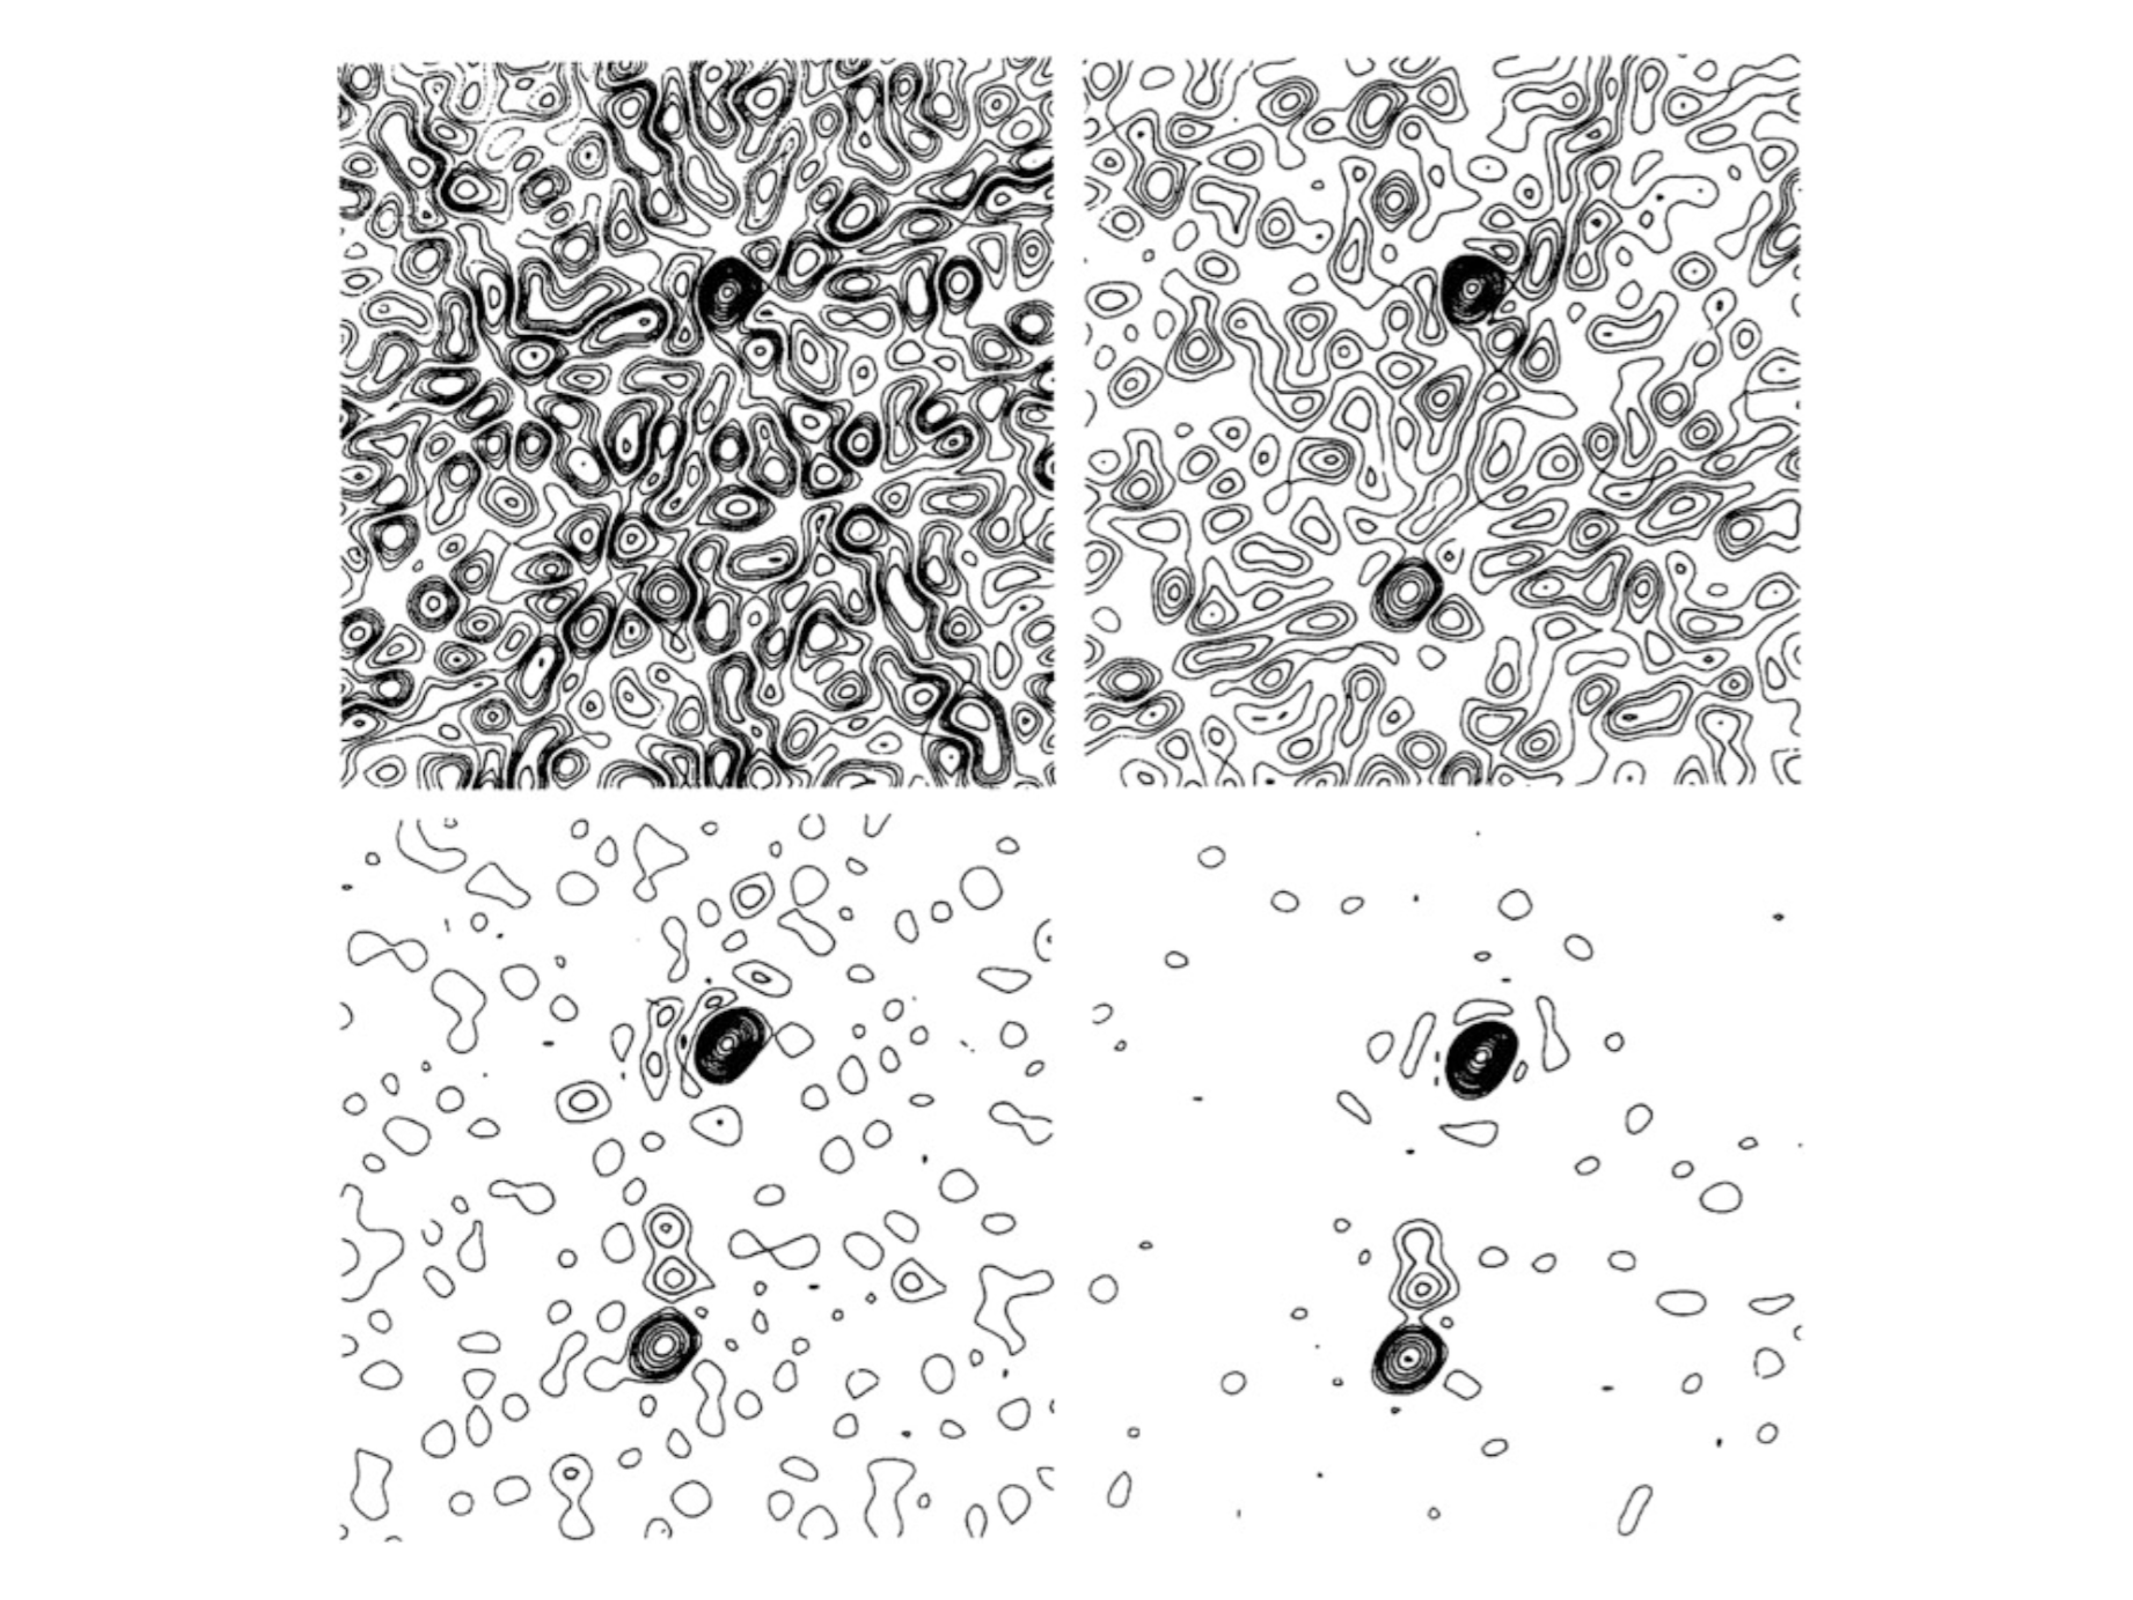
\includegraphics[width=0.85\textwidth]{chapters/interferometry/figures/gbt_clean.pdf}
\caption[Four stages of the H{\"o}gbom CLEAN.]{Four stages of the H{\"o}gbom CLEAN, as implemented on data from the Green Bank Interferometer. The top left panel shows the dirty image, with power scattered throughout the image plane. The top right panel shows the image after a single iteration with $\gamma=1$. The bottom left and bottom right panels show the image after two and six iterations, respectively. Contours are steps of 5\% from the maximum in each image. Figure taken from \cite{Hogbom.74, TMS}.}
\label{fig:gbt_clean_example}
\end{figure}

A major shortcoming of the H{\"o}gbom algorithm is its proliferation of small-scale structures around the locations of point sources. This is because the subtraction in Step 2, above, leaves new, local maxima around the perimeter of subtracted region. Later deconvolution algorithms, such as the one devised by \cite{Cornwell.83}, avoid this by padding the surrounding region according to an additional smoothness parameter. 

Imaging with extremely wide field-of-view instruments is explored in Chapter~\ref{chapter:polcal}.

\subsubsection{Delay Transforms and the 1D-CLEAN}

There are a variety of CLEANing techniques that are central to this thesis, but do not operate on images at all.
\cite{ParsonsBacker.09} and \cite{Parsons.12a} introduced the 1D-CLEAN, a deconvolution algorithm that operates on visibilities Fourier-transformed along the frequency axis, never gridding them on the $uv$-plane. Much more about Fourier-transformed visibilities will be spoken of throughout this work, and we discuss the basic points here.

A Fourier transform along the frequency axis of a visibility is called a `delay transform'. This nomenclature comes from the fact that Fourier conjugate of frequency is a quantity in units of time -- and the correct interpretation of this value is the time delay between a wavefront incident upon antenna $i$ and $j$. The delay $\tau_g$ of a source at (R.A.,Dec.)=($\alpha,\delta$) is

\begin{equation}
\tau_g = \frac{\vec{b}}{c}\cdot
\begin{pmatrix}
\cos\delta\cos({\rm h}-\alpha) \\
-\cos\delta\sin({\rm h}-\alpha) \\
\sin\delta \\
\end{pmatrix},
\end{equation}
for local sidereal time h. This value can be isolated in ``delay space" via a delay transform (where it is convenient to use the classical visibility equation for clarity, but all steps can be folded into the Jones formalism),

\begin{equation}
\begin{split}
\tilde{V}_{ij}(\tau, t) &= \int {\rm d}\nu g_i^*(\nu, t)g_j(\nu, t) V_{ij}(\nu,t)e^{2\pi i \nu \tau} \\
								   &= \int \tilde{g}_i(\tau, t)^*\tilde{g}_j(\tau, t) *
								   \sum_n^N \left[ \tilde{A}(\tau,\hat{s}_n(t)) * \tilde{S}_n(\tau) * \delta_D(\tau_g + \tau_{e,i,j} - \tau)\right]
\end{split}		   
\end{equation}
which is true for any polarization, so we have dropped our polarization indexing. Like the H{\"o}gbom algorithm, this explicitly assumes the sky can be expressed by $N$ point sources at positions $\hat{s}_n$. Instrumental absolute gains and phases are expressed as $g_i$, $g_j$ and $\tau_{e,i,j}= \tau_j - \tau_i$. Clearly, this procedure isolates a source $n$ as a delta function with amplitude $\tilde{S}_n$ at a given delay (assuming a smooth spectrum; see below), convolved by a kernel that describes the chromaticity of the instrument. If the instrument is designed to have a smooth frequency response, the $\tilde{g}_{i,j}(\tau)$ and $\tilde{A}(\tau)$ terms will be narrow functions in delay space and the value of $\tau_g + \tau_{e,i,j}$ will be well-constrained. If the instrument has an un-smooth spectral response, many more $\tau$-modes will be required to describe it, resulting in a spread of power in delay space. 

Figure~\ref{fig:delay_space_parsons12b} shows a graphical representation of a two-source sky model mapping from celestial coordinates to delay space. Note that the delay transform is not a one-to-one mapping -- sources in a plane perpendicular to the baseline vector share the same $\tau_g$. Dotted lines in the delay-space plot demarcate an extremely important value of $\tau$. A given baseline will have a \textit{maximum delay value}, $\tau_{\rm max} = |b|/c$, the light travel time between the antennas. With sufficient bandwidth and frequency resolution, this boundary can be clearly resolved, and all sources with smooth spectra (as is the case for unpolarized synchrotron radiation, but not for Faraday rotated polarized radiation or {\sc hi}; see Chapter~\ref{chapter:astro_rad} and almost all of Part II) will have their maximum power values within the $-\tau_{\rm max} \leqslant \tau \leqslant \tau_{\rm max}$ region.

\begin{figure}
\centering
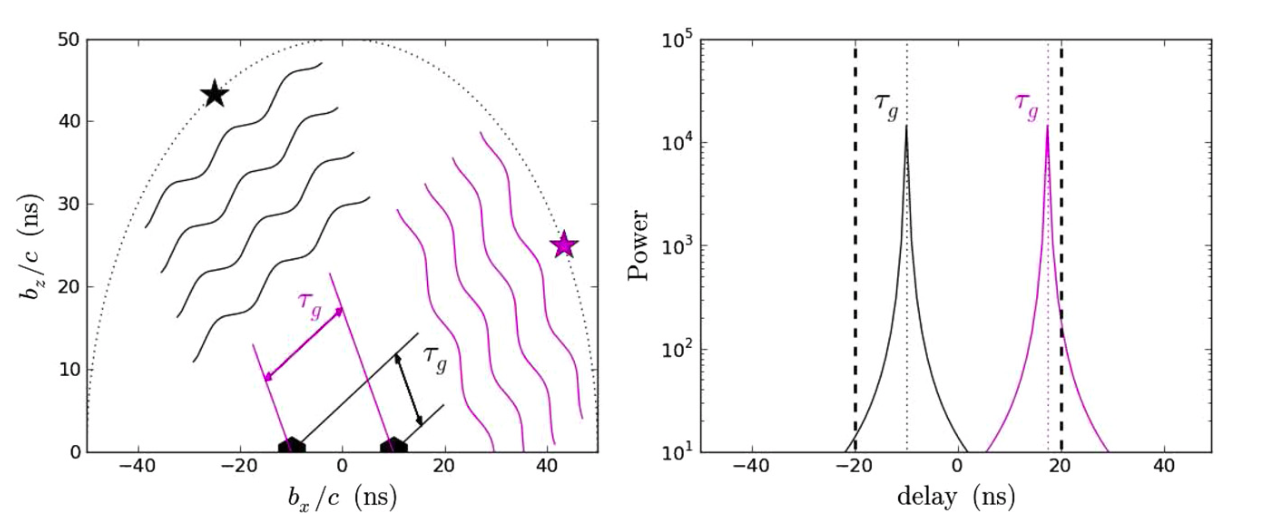
\includegraphics[width=0.8\textwidth]{chapters/interferometry/figures/delay_space_Parsons12b.png}
\caption[A graphical representation of the delay transform.]{A graphical representation of the delay transform. The left panel shows the relationship between celestial position and geometrical delay relative to a 60\,m baseline (which has a $\sim$20\,ns light-travel-time between antennas). The right panel shows an example delay transform of the visibilities recorded by this model interferometer. With perfect phase calibration, power from the sources is isolated to their geometrical delay, with some spread in delay space due to the chromaticity of the instrument. Figure taken from \cite{Parsons.12a}.} 
\label{fig:delay_space_parsons12b}
\end{figure}

By delay-transforming simulated visibilities with a simple sky model of the brightest sources and comparing to an observed sky with those sources close to zenith, one can estimate the instrumental delays and gains and obtain a delay-based calibration for $\textbf{J}_i^{\rm G}$. However, Fourier-transforming along an axis with discontinuities -- such as spikes or divets caused by Radio Frequency Interference (RFI) and its subsequenct flagging -- will result in sinc-like side lobes throughout delay space. Some interpolation is required to bridge these gaps, presented in \cite{ParsonsBacker.09} as the complex 1D-CLEAN. The algorithm proceeds as follows:

\begin{enumerate}
\item Delay-transform the visibility containing nulled frequency channels -- this is the ``dirty image".
\item As in the H{\"o}gbom algorithm, iteratively propagate the largest magnitude feature, by $\tau$ bin, to a model after convolving it with the Fourier transform of the flags themselves -- this is the ``dirty beam".
\item Stop when the residual power in delay space is beneath some defined threshold. Add this residual power to the model.
\end{enumerate}

The importance of the delay transform for EoR studies is discussed in Chapter~\ref{chapter:eor_window_theory}, and a variant of it is presented in Chapter~\ref{chapter:eor_window_psa128}.

\subsection{Redundant calibration}

Thus far we have discussed calibration techniques that require some model of the sky to begin with. For an interferometer without any repeated baseline vectors, these methods are sufficient. However, some EoR studies, such as those discussed in this thesis, have opted to construct highly redundant arrays, with many repeated baselines. Such interferometers sample comparatively few modes of the $uv$-plane, leading to poor images -- but their visibilities can be averaged together in order to reduce noise for EoR measurements on specific spatial scales.

We defer detailed discussion of redundant calibration to Chapter~\ref{chapter:polcal}, but provide a brief overview here (studies that explore this technique in depth include \cite{Wieringa.92, Liu.10, Zheng.14} and \cite{Dillon.17}). In a redundant array, there are several examples of a given ``visibility type". Assuming the antennas have identical beams (understanding non-redundant beams is a contemporary effort), the only difference between the visibilities should be due to their complex gains. For a visibility type $V^{pq}_{|i-j|}(\nu, t)$, all baselines with baseline vector $\vec{b}_{|i-j|}$ may be described as 

\begin{equation}
V_{ij}(\nu, t) = g^{p*}_i(\nu, t)  g^{q}_j(\nu, t) V^{pq}_{|i-j|}(\nu, t) + n_{ij}(\nu,t),
\label{eq:interferometry_redcal}
\end{equation}
where the $n_{ij}$ term represents noise on that visibility. For a redundant array, this system of equations is highly overdetermined to solve for $g^p_i$ and $ g^{q}_j$, as long as $V^{pq}_{|i-j|}$ can be formed (this can simply be the median of all of the visibilities of that type in the data). Again, for a fuller mathematical overview we defer to Chapter~\ref{chapter:polcal}.

We have made the frequency and time dependence explicit in order to emphasize that the complex gains can be solved-for each every frequency,time sample. This is unlike the delay transform (which requires a frequency bandwidth to transform over) or imaging calibration (which can in principle be implemented per-time and frequency, but is difficult due to the resultant very noisy dirty images). 

Using redundant calibration, when available, can reduce the number of diagonal gains to solve for from $\frac{1}{2}N_{\rm ants}(N_{\rm ants} - 1)$ to just a few unknowns. These unknowns are degeneracies of the system of equations defined in Equation~\ref{eq:interferometry_redcal}, and arise from the fact that no information from the sky is required to obtain diagonal gains that are self-consistent between antennas. For the simplest implementation of such a system, as presented in \cite{Zheng.14}, there are four degeneracies per feed arm (so eight overall). These are:

\begin{itemize}
\item Overall amplitude scaling (to obtain the correct flux density of the sky),
\item Overall phasing (an arbitrary additional phase ramp),
\item Phasing along the $\hat{\theta}$ direction (correct positions on the sky),
\item Phasing along the $\hat{\phi}$ direction (correct positions on the sky).
\end{itemize}

These additional parameters can be obtained by making an image of a calibration field -- no CLEANing should be required, since power should be self-consistently distributed in the $uv$-plane -- where the sky will likely be incorrectly centered and of incorrect amplitude.

\section{Instrumental Polarization}
\label{sec:interferometry_pol}
% pseudo-Stokes as sum of Mueller terms

An interferometer is capable of measuring pseudo-Stokes visibilities, which contain components of Stokes power, somehow convolved by the instrumental response. Understanding this instrumental response is crucial for performing polarimetry at low frequencies. As we will see, the instrument will inherently `leak' power between polarizations in direction dependent (effects that occur inside the visibility integral) and independent (outside of the visibility integral) ways. These leakage modes must be well-understood in order to make any statements about the nature of the polarized sky.

Synthesizing the Jones formalism introduced in Section~\ref{sec:interferometry_vis} and the calibration terms in Section~\ref{sec:interferometry_cal}, we seek to understand how the Jones chain,

\begin{equation}
\textbf{J}_i = \textbf{J}_i^{\rm D}(\nu) \textbf{J}_i^{\rm G}(\nu)  \textbf{J}_i^{\rm I}(\hat{s},\nu) \textbf{J}_i^{\rm \Gamma}(\hat{s},\nu)  \textbf{J}_i^{\rm B}(\hat{s},\nu) ,
\end{equation}
influences the power in pseudo-Stokes visibilities.

\subsection{Direction-Dependent Leakage}

The direction-dependent terms in the Jones chain concern the beam, and ionospheric effects. In this section, we will concentrate on the beam Jones matrix -- the ionospheric effects are discussed in detail elsewhere \citep[e.g.][{\color{red} Martinot et al. (in prep.)}]{Intema.09,Vedantham.15,Vedantham.16}.

Unless $\textbf{J}_i^{\rm B}(\hat{s},\nu)$ is both diagonal and, at any given point on the sphere, the diagonal elements are equal, there will be mixing or ``leaking" of different Stokes parameters together into each element of $\textbf{V}_{ij}$ in a direction dependent way \citep[e.g.][]{Geil.11, Smirnov.11, Smirnov.11.2, Nunhokee.17}. Focusing on pseudo-Stokes I and neglecting other Jones terms for a moment,

\begin{equation}
\begin{split}
V^I_{ij}(\nu) &= {\rm Tr}(\textbf{V}_{ij}) = \int {\rm Tr}(\textbf{J}_i^{\rm B}\textbf{C}_{ij}\textbf{J}_j^{{\rm B}H}) \exp(-2\pi i \nu \vec{b}\cdot\hat{s}/c) {\rm d}\Omega \\
					  &= \int \textbf{M}_{00}I + \textbf{M}_{01}Q + \textbf{M}_{02}U + \textbf{M}_{03}V \exp(-2\pi i \nu \vec{b}\cdot\hat{s}/c) {\rm d}\Omega
\end{split}
\label{eq:interferometry_pseudo-stokes-I-leakage}
\end{equation}
where I, Q, U and V are the true Stokes sky and are functions of direction and frequency, and the $\textbf{M}_{ab}$ terms are components of the direction dependent instrumental Mueller matrix, also functions of direction and frequency:

\begin{equation}
\textbf{M}_{ab}(\hat{s},\nu) = {\rm Tr} ( \sigma_a \textbf{J}_i^{\rm B} \sigma_b \textbf{J}_j^{{\rm B}H})
\label{eq:interferometry_mueller-terms}
\end{equation}
and $\sigma_k$ are the Pauli matrices, where the indices are reordered from the quantum mechanical convention such that 

\begin{equation}
\begin{split}
\sigma_0 &=\begin{pmatrix}1 & 0 \\0 & 1 \\ \end{pmatrix},\,
\sigma_1 = \begin{pmatrix} 1 & 0 \\ 0 & -1 \\ \end{pmatrix},\,
\sigma_2 = \begin{pmatrix} 0 & 1 \\ 1 & 0 \\ \end{pmatrix},\,
\sigma_3 = \begin{pmatrix} 0 & -i \\ i & 0 \\ \end{pmatrix} \\\\
V^I &= {\rm Tr}\left( \sigma_0\textbf{V} \right),\, V^Q= {\rm Tr}\left( \sigma_1\textbf{V} \right),\, V^U = {\rm Tr}\left( \sigma_2\textbf{V} \right),\, V^V = {\rm Tr}\left( \sigma_3\textbf{V} \right).
\end{split}
\end{equation}

Equation~\ref{eq:interferometry_pseudo-stokes-I-leakage} explicitly shows that the pseudo-Stokes I visibility is inherently composed of the weighted sum of all of the Stokes parameters, where the weighting is direction- and frequency-dependent, given by the Mueller terms  $\textbf{M}_{ab}(\hat{s},\nu)$ in Equation~\ref{eq:interferometry_mueller-terms}. In turn, the $\textbf{M}_{ab}(\hat{s},\nu)$ terms are completely determined by the beam Jones matrix; a collection of complex voltage beam patterns. With a simulated instrument, one can obtain the $4\times 4$ $\textbf{M}(\hat{s},\nu)$ matrix and model the contribution of each Stokes parameter to each pseudo-Stokes visibility. The key to such a Mueller matrix is

\begin{equation}
\mathcal{M}_{ab}(\hat{s},\nu) =
\begin{pmatrix}
I \rightarrow V^I & I \rightarrow V^Q & I \rightarrow V^U & I \rightarrow V^V\\
Q \rightarrow V^I  & Q \rightarrow V^Q & Q \rightarrow V^U & Q \rightarrow V^V\\
U \rightarrow V^I  & U \rightarrow V^Q & U \rightarrow V^U & U \rightarrow V^V\\
V \rightarrow V^I  & V \rightarrow V^Q & V \rightarrow V^U & V \rightarrow V^V\\
\end{pmatrix}
\label{eq:interferometry_Mab}
\end{equation}

\cite{Fagnoni.16} simulated the feed, faceted parabolic dish and analog signal chain for the Hydrogen Epoch of Reionization Array (HERA) instrument using the CST\footnote{\url{www.cst.com}} package. They generated the $\vec{E}$-field receptivity patterns that could be used to form $\textbf{J}_i^{\rm B}$ and $\textbf{M}(\hat{s},\nu)$. Examples of $\textbf{M}(\hat{s},\nu)$ at 120\,MHz and 160\,MHz are shown in Figure~\ref{fig:interferometry_Mab}, projected in the R.A., Dec. basis. Note that this basis has a singularity at the South Pole, leading to wide-field asymmetries in components to do with Stokes Q and U. Due to the large spread in dynamic ranges between $\textbf{M}_{00}$, other diagonal terms, and off-diagonal terms, we use separate color maps for each. All of the dynamic ranges are normalized to the peak of $\textbf{M}_{00}$, which is 1 at zenith. The off-diagonal terms are 2- to 8-orders of magnitude less than the diagonal terms.

\begin{figure}
\centering
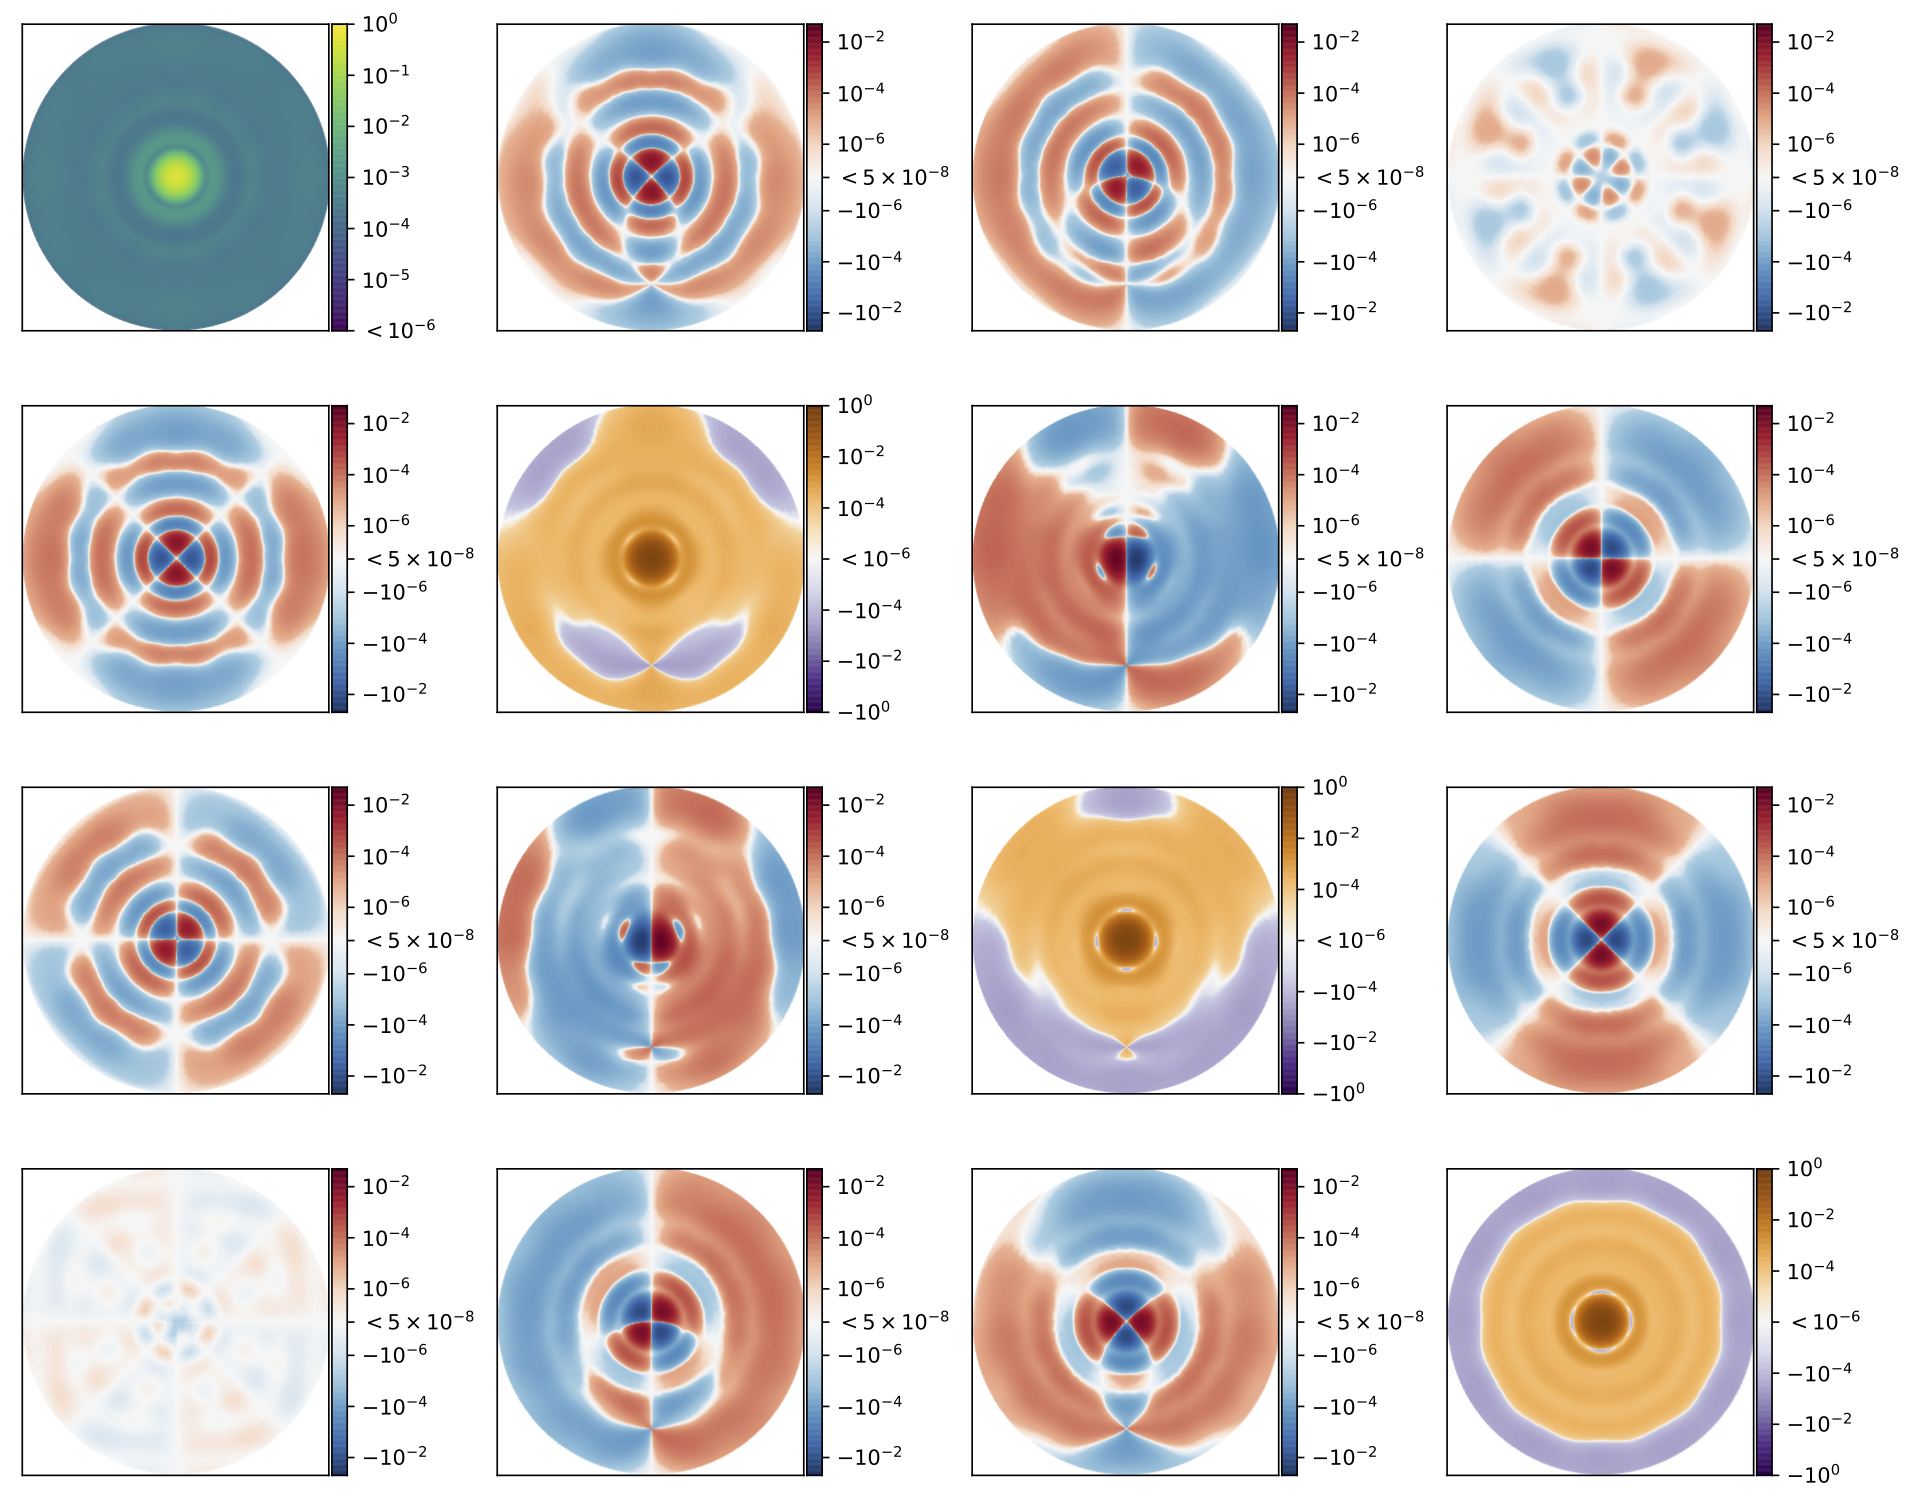
\includegraphics[width=0.7\textwidth]{chapters/interferometry/figures/full_mueller_120MHz.png}
\par\noindent\rule{0.8\textwidth}{0.4pt}
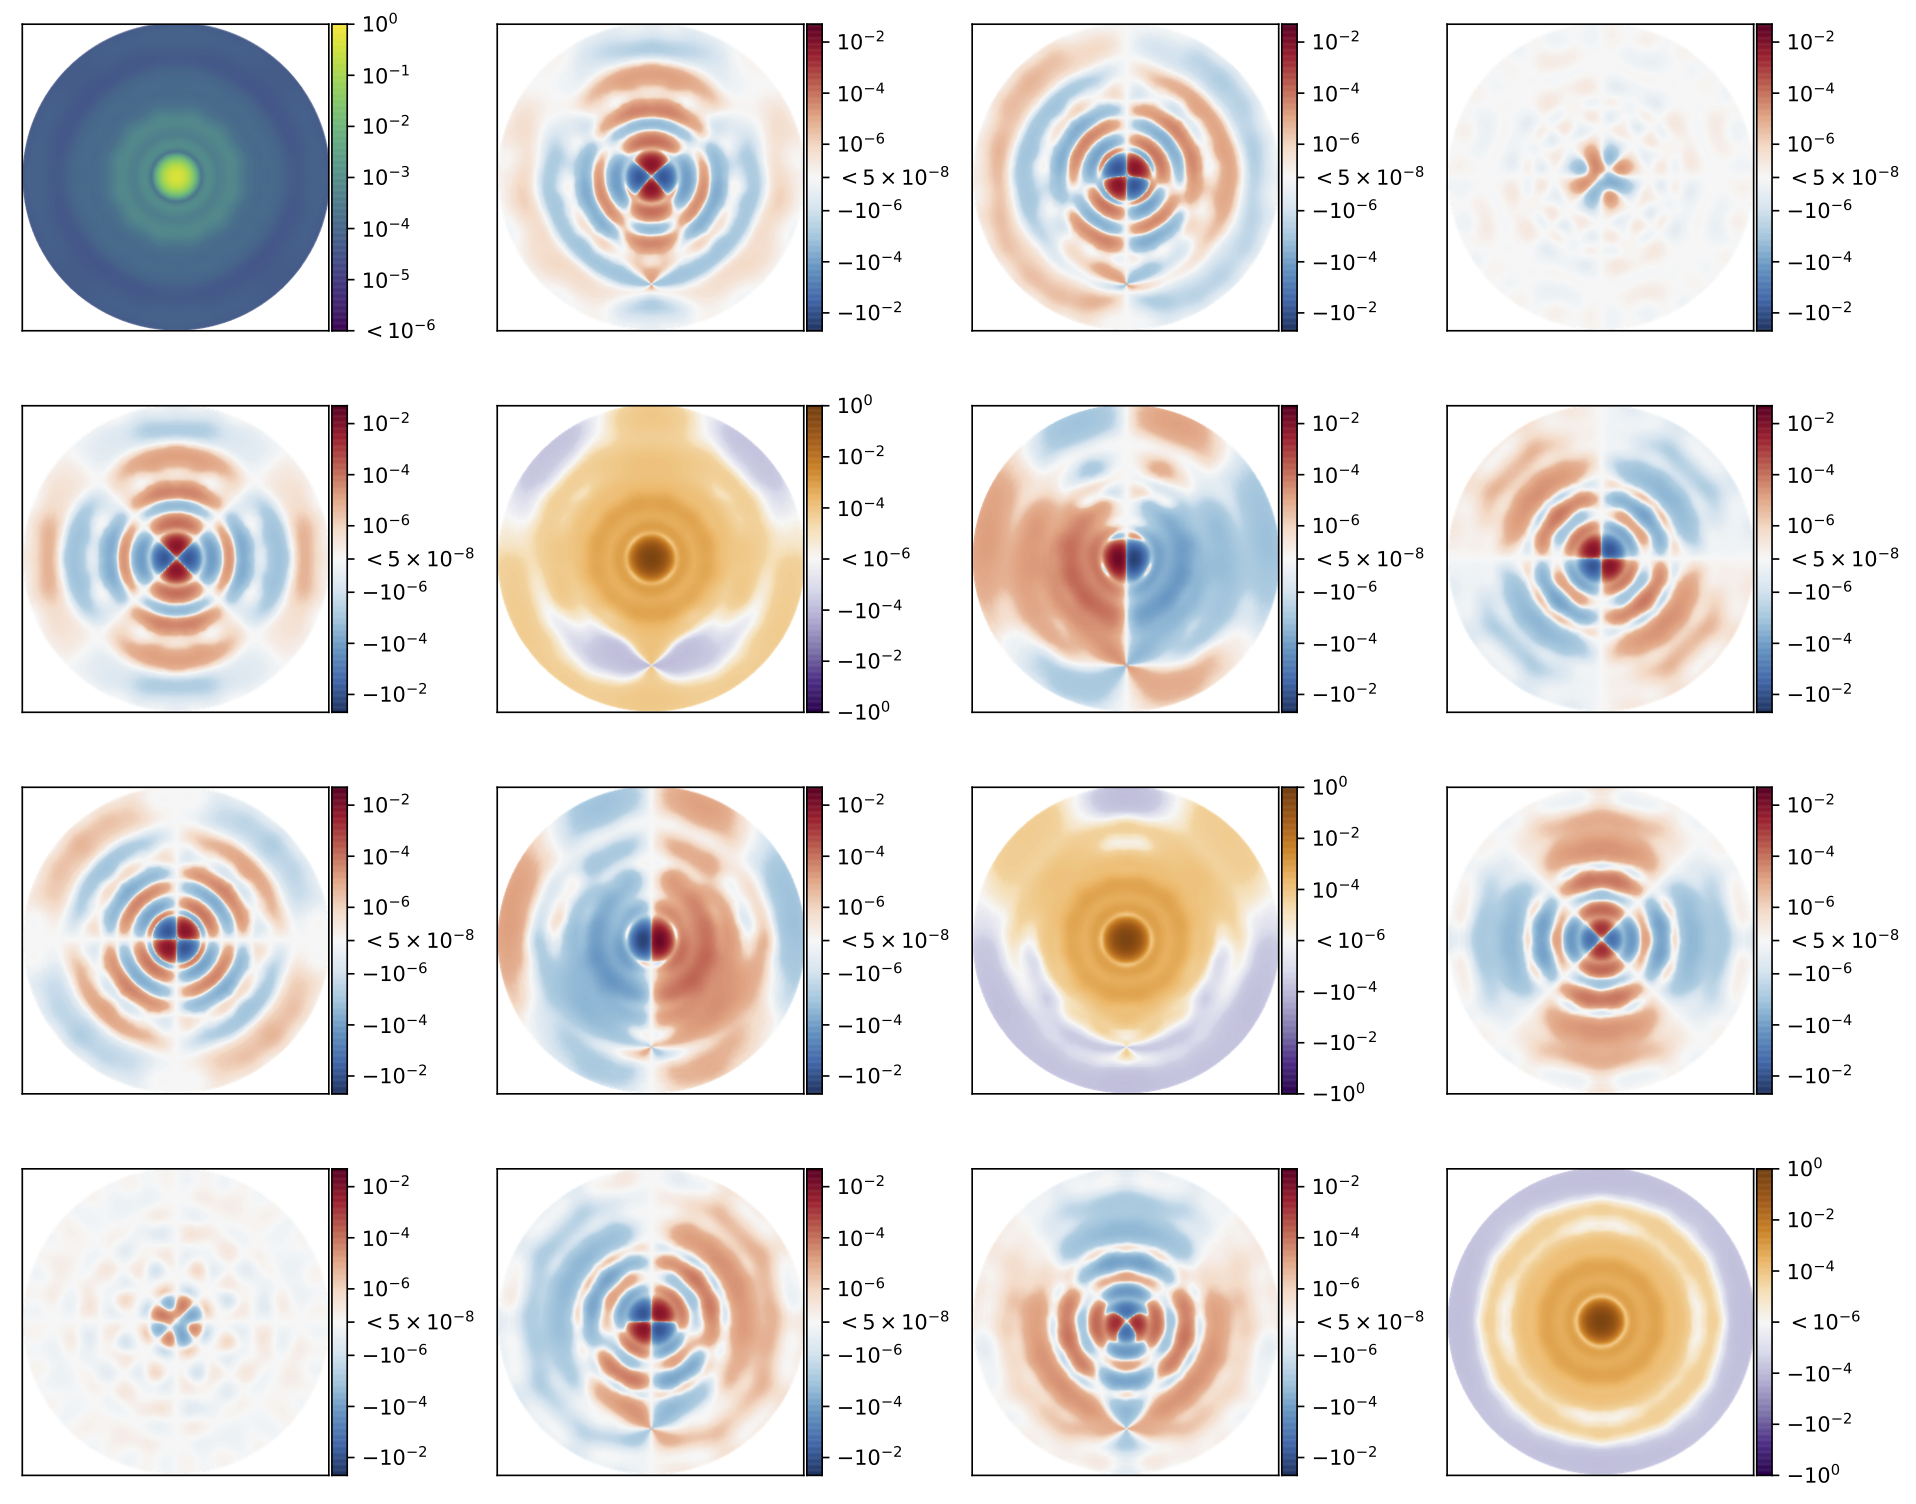
\includegraphics[width=0.7\textwidth]{chapters/interferometry/figures/full_mueller_160MHz.png}
\caption[Simulations of the instrumental direction-dependent Mueller matrix at 120 MHz and 160 MHz.]{Simulations of the instrumental direction dependent Mueller matrix at 120 MHz and 160 MHz (\textit{above} and \textit{below}, respectively) projected into the RA, Dec basis. Color scales for frequencies are relative to the peak of $\textbf{M}_{00}$ (which itself is normalized to 1 at zenith). To account for the wide variety of dynamic ranges required to show detail, we use separate color maps for $\textbf{M}_{00}$, diagonal, and off-diagonal terms. The off-diagonal terms are 2- to 8-orders of magnitude less than the diagonal terms. For a key to these matrices, see Equation~\ref{eq:interferometry_Mab}.}
\label{fig:interferometry_Mab}
\end{figure}

As discussed in Chapter~\ref{chapter:astro_rad}, at the low frequencies and large scales relevant to EoR experiments, the Stokes I sky is extremely bright compared to the other Stokes parameters, and few polarized point sources have been found. This makes the first column of $\textbf{M}(\hat{s},\nu)$, representing $I\,\rightarrow\,V^I\,V^Q\,V^U\,V^V$ the most interesting for characterizing the polarized response of an instrument observationally. It can be reasonably expected that even a small amount of leakage from Stokes I into the other Stokes parameters will dominate over Stokes Q, U and V power alone.

Deconvolution of $\textbf{M}(\hat{s},\nu)$ for wide field-of-view instruments is not at all a solved problem, with contemporary studies ``learning to live with it". Hypothetically, with accurate polarized sky and instrument models, one could use the linear nature of the Jones formalism to compute each ``visibility component",

\begin{equation}
\hat{V}^{ab}_{ij} = \int \textbf{M}_{ab}(\hat{s},\nu)S_P(\hat{s},\nu)\exp(-2\pi i \nu \vec{b}\cdot\hat{s}/c) {\rm d}\Omega,
\end{equation}
where $S_P \in (I, Q, U, V)$. Subtracting the additional components from a given pseudo-Stokes visibility could isolate that Stokes parameter. While accurate instrument models are presently becoming available (see Chapter~\ref{chapter:eor_window_HERA} for verification of the simulations shown in Figure~\ref{fig:interferometry_Mab}, at least for pseudo-Stokes I), verifying the accuracy of such a method would require precise expectations of the nature of the low frequency polarized sky. At the time of writing, this is only beginning to become clear through polarized sky surveys from the Low Frequency Array (LOFAR; e.g. \citet{VanEck.18}) and the MWA \citep[e.g.][]{Lenc.16, Lenc.17}.

\subsection{Direction-Independent Leakage}

In addition to the mixing of Stokes parameters due to the primary beam, it is possible to mix them in a direction independent way. Calibration errors -- errors in the estimation of the components of $\textbf{J}_i^{\rm D}(\nu)$ and $\textbf{J}_i^{\rm G}(\nu)$ -- are capable of leaking signal between pseudo-Stokes visibilities independent of the sky. Writing the gains as $g_i^p(\nu) + \delta g_i^p(\nu)$, and $\textbf{J}_i (\nu)=\textbf{J}_i^{\rm D}(\nu)\textbf{J}_i^{\rm G}(\nu)$,  a direction-independent Mueller matrix may be composed \citep{TMS}:

\begin{equation}
\textbf{M}'(\nu) = \textbf{J}_i (\nu) \otimes \textbf{J}_j^H (\nu)
\end{equation}
such that

\begin{equation}
\begin{pmatrix}
V'_I \\
V'_Q \\
V'_U \\
V'_V \\
\end{pmatrix}
=
(\textbf{I} - \frac{1}{2}\delta\textbf{M}')
\begin{pmatrix}
V_I \\
V_Q \\
V_U \\
V_V \\
\end{pmatrix}
\end{equation}
where

\begin{table}[h!]
\setcounter{MaxMatrixCols}{4}
\renewcommand\arraystretch{1.25}
\resizebox{\textwidth}{!}{$
\delta\textbf{M}' = 
\begin{pmatrix}
\delta g_i^p + \delta g_i^q + \delta g_j^{p*} +  \delta g_j^{q*} &
\delta g_i^p - \delta g_i^q + \delta g_j^{p*} -  \delta g_j^{q*} &
D_i^p - D_i^q + D_j^{p*} - D_j^{q*} &
-\textbf{i}( D_i^p + D_i^q - D_j^{p*} - D_j^{q*} ) \\
\delta g_i^p - \delta g_i^q + \delta g_j^{p*} -  \delta g_j^{q*}  &
\delta g_i^p + \delta g_i^q + \delta g_j^{p*} +  \delta g_j^{q*} &
D_i^p + D_i^q + D_j^{p*} + D_j^{q*} & 
-\textbf{i}(D_i^p - D_i^q - D_j^{p*} + D_j^{q*})\\
D_i^p - D_i^q + D_j^{p*} - D_j^{q*} &
- (D_i^p + D_i^q + D_j^{p*} + D_j^{q*}) &
\delta g_i^p + \delta g_i^q + \delta g_j^{p*} +  \delta g_j^{q*} &
\textbf{i}(\delta g_i^p - \delta g_i^q - \delta g_j^{p*} +  \delta g_j^{q*})\\
-\textbf{i}(D_i^p + D_i^q - D_j^{p*} - D_j^{q*}) &
-\textbf{i}(D_i^p - D_i^q - D_j^{p*} + D_j^{q*}) &
\textbf{i}(\delta g_i^p - \delta g_i^q - \delta g_j^{p*} +  \delta g_j^{q*}) &
\delta g_i^p + \delta g_i^q + \delta g_j^{p*} +  \delta g_j^{q*} \\
\end{pmatrix}$}
\end{table}
where we have approximated the components to first order in $\delta g$ and $D$, dropped the frequency dependence of each term, and \textbf{i} indicates the imaginary unit. $V'_I$ denotes the observed value of the pseudo-Stokes I visibility. In the regime of leaked pseudo-Stokes I power dominating over pseudo-Stokes Q, U and V, this shows that pseudo-Stokes I appears in pseudo-Stokes Q through errors in diagonal gain calibration, and pseudo-Stokes U and V through uncalibrated \textit{D}-terms.

A fraction of the \textit{D}-term leakage from pseudo-Stokes I into U and V may approximated by a delay between the $p$ and $q$ feeds, $\tau_{pq}$. This is a valid approximation, as a time delay between a wavefront incident upon two feed arms is exactly what circular polarization is, so signal appearing in Stokes V should be able to be described in this form. In Chapter~\ref{chapter:eor_window_paper32img} we present a fit for this parameter across the array, and find that through such a fit pseudo-Stokes V signal can be transferred to pseudo-Stokes U. In Chapter~\ref{chapter:polcal}, we present a method that combines such a fit with redundant calibration, allowing us to minimize leaked power into pseudo-Stokes V on a per-time and -frequency sample basis.\\\\

This Chapter has reviewed the fundamentals of radio interferometry, providing a formalism generalized to wide field-of-view observations, and polarization. The importance of understanding the polarized response of the instrument has been emphasized many times. In the Part II, this emphasis will be justified from several data- and theory-based approaches.
